\documentclass{article}
\usepackage{amsmath}
\usepackage{graphicx}
\usepackage{listings}
\usepackage{xcolor}
\usepackage{float}

\lstdefinestyle{matlabstyle}{
    language=Matlab,
    basicstyle=\ttfamily\small,
    numberstyle=\tiny,
    numbers=left,
    numbersep=5pt,
    showstringspaces=false,
    breaklines=true,
    frame=single,
    frameround=tttt,
    backgroundcolor=\color{gray!5},
    commentstyle=\color{green!60!black},
    keywordstyle=\color{blue!80!black},
    stringstyle=\color{purple!40!black},
    emphstyle=\color{red!60!black},
    emph={subplot,stairs,xlabel,ylabel,axis,legend,hold},
    morekeywords={clear,clc},
    captionpos=b,
    aboveskip=1.5\baselineskip,
    belowskip=1.5\baselineskip,
    columns=flexible,
    keepspaces=true
}

\usepackage[top=2cm, bottom=2cm, left=2.5cm, right=2.5cm]{geometry}
\usepackage{amsmath}

\begin{document}

\title{Program Robot Sepak Bola Manual}
\author{Figo Arzaki Maulana - 5022221041}
\date{Rabu, 17 Maret 2025}
\maketitle
\section{Penjelasan Program Robot Sepak Bola}

Program ini merupakan implementasi sistem kendali robot diferensial Pioneer P3DX yang digunakan dalam simulasi CoppeliaSim.

\subsection{Parameter Robot}
Robot memiliki dua parameter fisik utama yaitu radius roda (R) sebesar 0,0975 meter dan jarak antar roda (L) sebesar 0,381 meter. Program mengimplementasikan sistem debouncing dengan waktu tunda 0,1 detik untuk mencegah input berulang yang tidak diinginkan saat tombol ditekan.

\subsection{Sistem Kendali}
Sistem kendali robot menggunakan inverse kinematics untuk mengkonversi kecepatan linear dan angular yang diinginkan menjadi kecepatan rotasi masing-masing roda. Fungsi inverseKinematics menggunakan matriks inverse untuk menghitung kecepatan roda kanan dan kiri berdasarkan input kecepatan yang diberikan.

\subsection{Implementasi Kontrol}
Kontrol robot dilakukan melalui keyboard dengan tombol panah. Tombol panah atas dan bawah mengatur kecepatan linear (maju/mundur) dengan perubahan 0,1 unit setiap penekanan, sedangkan tombol panah kiri dan kanan mengatur kecepatan angular (berbelok) dengan perubahan yang sama. Program membatasi kecepatan linear maksimum pada 1 m/s dan kecepatan angular maksimum pada 0,5 rad/s untuk menjaga stabilitas pergerakan robot. tombol reset (R) dapat mengembalikan kecepatan ke nilai nol.

\section{Diagram Kontrol}
\begin{figure}[h]
    \centering
    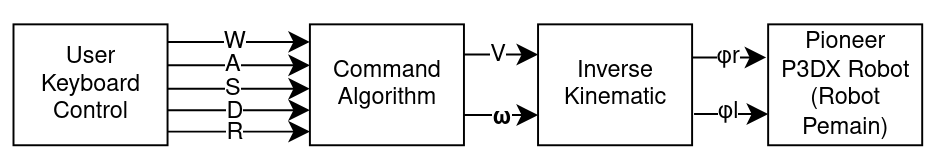
\includegraphics[width=0.8\textwidth]{control.png}
    \caption{Diagram Kontrol Robot}
    \label{fig:control}
\end{figure}
\newpage
\section{Kode Program}

\begin{lstlisting}[style=matlabstyle]

    from coppeliasim_zmqremoteapi_client import RemoteAPIClient
    import keyboard
    import time
    import numpy as np
    
    R = 0.0975 # radius of the wheel
    L = 0.381 # distance between the wheels
    DEBOUNCE_TIME = 0.1  # 100ms debounce time
    last_key_press = {
        "up": 0,
        "down": 0,
        "left": 0,
        "right": 0,
        "r": 0
    }
    
    def inverseKinematics(v, w):
        inverse_matrix = np.linalg.inv(np.array([[R/2, R/2], [R/(2*L), -R/(2*L)]]))
        return np.dot(inverse_matrix, [v, w])
    
    def getMotorsHandle():
        motorRightHandle = sim.getObject("/Robot_Pemain/rightMotor")
        motorLeftHandle = sim.getObject("/Robot_Pemain/leftMotor")
        return (motorRightHandle, motorLeftHandle)
    
    def setRobotMotion(motorsHandle, veloCmd):
        _ = sim.setJointTargetVelocity(motorsHandle[0], veloCmd[0])
        _ = sim.setJointTargetVelocity(motorsHandle[1], veloCmd[1])
        return
    
    client = RemoteAPIClient()
    sim = client.require("sim")
    
    sim.setStepping(False)
    sim.startSimulation()
    
    motors_handle = getMotorsHandle()
    
    cmd_vel = [0.0, 0.0]
    prev_cmd_vel = [0.0, 0.0]
    wheel_vel = [0.0, 0.0]
    lin_vel_lim = 1
    ang_vel_lim = 0.5
    
    while True:
        if keyboard.is_pressed("esc"):
            break
        
        current_time = time.time()
        if keyboard.is_pressed("up") and (current_time - last_key_press["up"]) > DEBOUNCE_TIME:
            cmd_vel[0] += 0.1
            last_key_press["w"] = current_time
        if keyboard.is_pressed("down") and (current_time - last_key_press["down"]) > DEBOUNCE_TIME:
            cmd_vel[0] -= 0.1
            last_key_press["s"] = current_time
        if keyboard.is_pressed("left") and (current_time - last_key_press["left"]) > DEBOUNCE_TIME:
            cmd_vel[1] += 0.1
            last_key_press["a"] = current_time
        if keyboard.is_pressed("right") and (current_time - last_key_press["right"]) > DEBOUNCE_TIME:
            cmd_vel[1] -= 0.1
            last_key_press["d"] = current_time
        if keyboard.is_pressed("r") and (current_time - last_key_press["r"]) > DEBOUNCE_TIME:
            cmd_vel = [0.0, 0.0]
            last_key_press["r"] = current_time
        
        if cmd_vel[0] > lin_vel_lim:
            cmd_vel[0] = lin_vel_lim
        if cmd_vel[0] < -lin_vel_lim:
            cmd_vel[0] = -lin_vel_lim
        if cmd_vel[1] > ang_vel_lim:
            cmd_vel[1] = ang_vel_lim
        if cmd_vel[1] < -ang_vel_lim:
            cmd_vel[1] = -ang_vel_lim 
        
        wheel_vel = inverseKinematics(cmd_vel[0], cmd_vel[1])
        
        if cmd_vel != prev_cmd_vel:
            print(f"cmd_vel: {cmd_vel}, wheel_vel: {wheel_vel}")
        
        setRobotMotion(motors_handle, wheel_vel)
        prev_cmd_vel = cmd_vel.copy()
    
    
    sim.stopSimulation()
    print("\nProgram Ended\n")
\end{lstlisting}
  

\end{document}